\chapter{Analisis}


\section{Analisis Frontend Library}
\subsection{Foundation}
Dalam projek BlueTape, file Foundation tersimpan di folder js dan css. Foundation yang digunakan pada projek ini adalah versi 6.1.2. Detail dari file - file dalam folder css sebagai berikut :
\begin{enumerate}		
	\item \verb|foundation-flex.css| : Penggunaan Flex Grid yang dipakai sebelum versi 6.4.
	\item \verb|foundation-icons.css| : Terdiri dari semua ikon yang dimiliki Foundation.
	\item \verb|foundation-icons.eot|, \verb|foundation-icons.svg|, \verb|foundation-icons.ttf|, \verb|foundation-icons.woff| : Serangkaian file stylesheets untuk menunjang penggunaan web fonts.
	\item \verb|foundation.css| : File foundation yang berisi desain default dari framework Foundation. 
\end{enumerate}	
Detail dari file - file dalam folder js sebagai berikut :
\begin{enumerate}
	\item Folder vendor : terdiri dari file \verb|jquery.min.js| dan \verb|what-input.min.js| yaitu file jQuery yang digunakan untuk membangun framework dengan Foundation.
	\item \verb|app.js| : Berisi fungsi untuk menginisiasi semua plugin pada Foundation.
	\item \verb|foundation.js| : Berisi semua file javascript dari framework Foundation.
\end{enumerate}
\subsection{Xdan datetime picker}
Penggunaan plugin date time picker pada Foundation disimpan pada folder lib/xdan-datetimepicker dan css :
\begin{enumerate}
	\item \verb|foundation-datepicker.min.css| : File berisi pengaturan desain dari penggunaan plugin datepicker yang disimpan pada folder css.
	\item \verb|jquery.datepickerpicker.full.min.css| : browser file
	\item \verb|jquery.datepickerpicker.min.css| : browser minified file
	\item \verb|jquery.datepickerpicker.min.js| : amd module style minified file	
\end{enumerate}

\section{Analisis views}
\subsection{Folder Templates}
Website BlueTape terdiri dari beberapa template yang disimpan di path BlueTape/www/application/views/template yaitu:
\begin{enumerate}
	\item \verb|flashmessage.php| : Template berisi kode php yang akan memberi tahu user apabila proses yang dilakukan terjadi error atau memiliki informasi tertentu. kelas \verb|alert| dibutuhkan untuk kebutuhan tampilan notifikasi.	
	\item \verb|head_loggedin.php| : Bagian \texttt{<head>} yang medefinisikan seluruh file css beserta plugin yang digunakan. Disini nantinya akan didefinisikan file css dari bootstrap dan plugin \textit{date-time-picker} dari bootstrap.
	\item \verb|script_foundation| : Bagian yang mendefinisikan seluruh file javascript yang digunakan oleh framework.  Disini nantinya akan didefinisikan file js dari bootstrap dan plugin \textit{date-time-picker} dari bootstrap.
	\item \verb|topbar_loggedin.php| : Template berisi navigation bar yang terdiri menu - menu. Dibutuhkan kelas \verb|navbar| dan kelas \verb|form-inline| untuk membuat sebuah navigation bar yang memiliki menu - menu yang sebaris.
\end{enumerate}

\subsection{Antarmuka Login}
\begin{figure} [H]	
	\centering  
	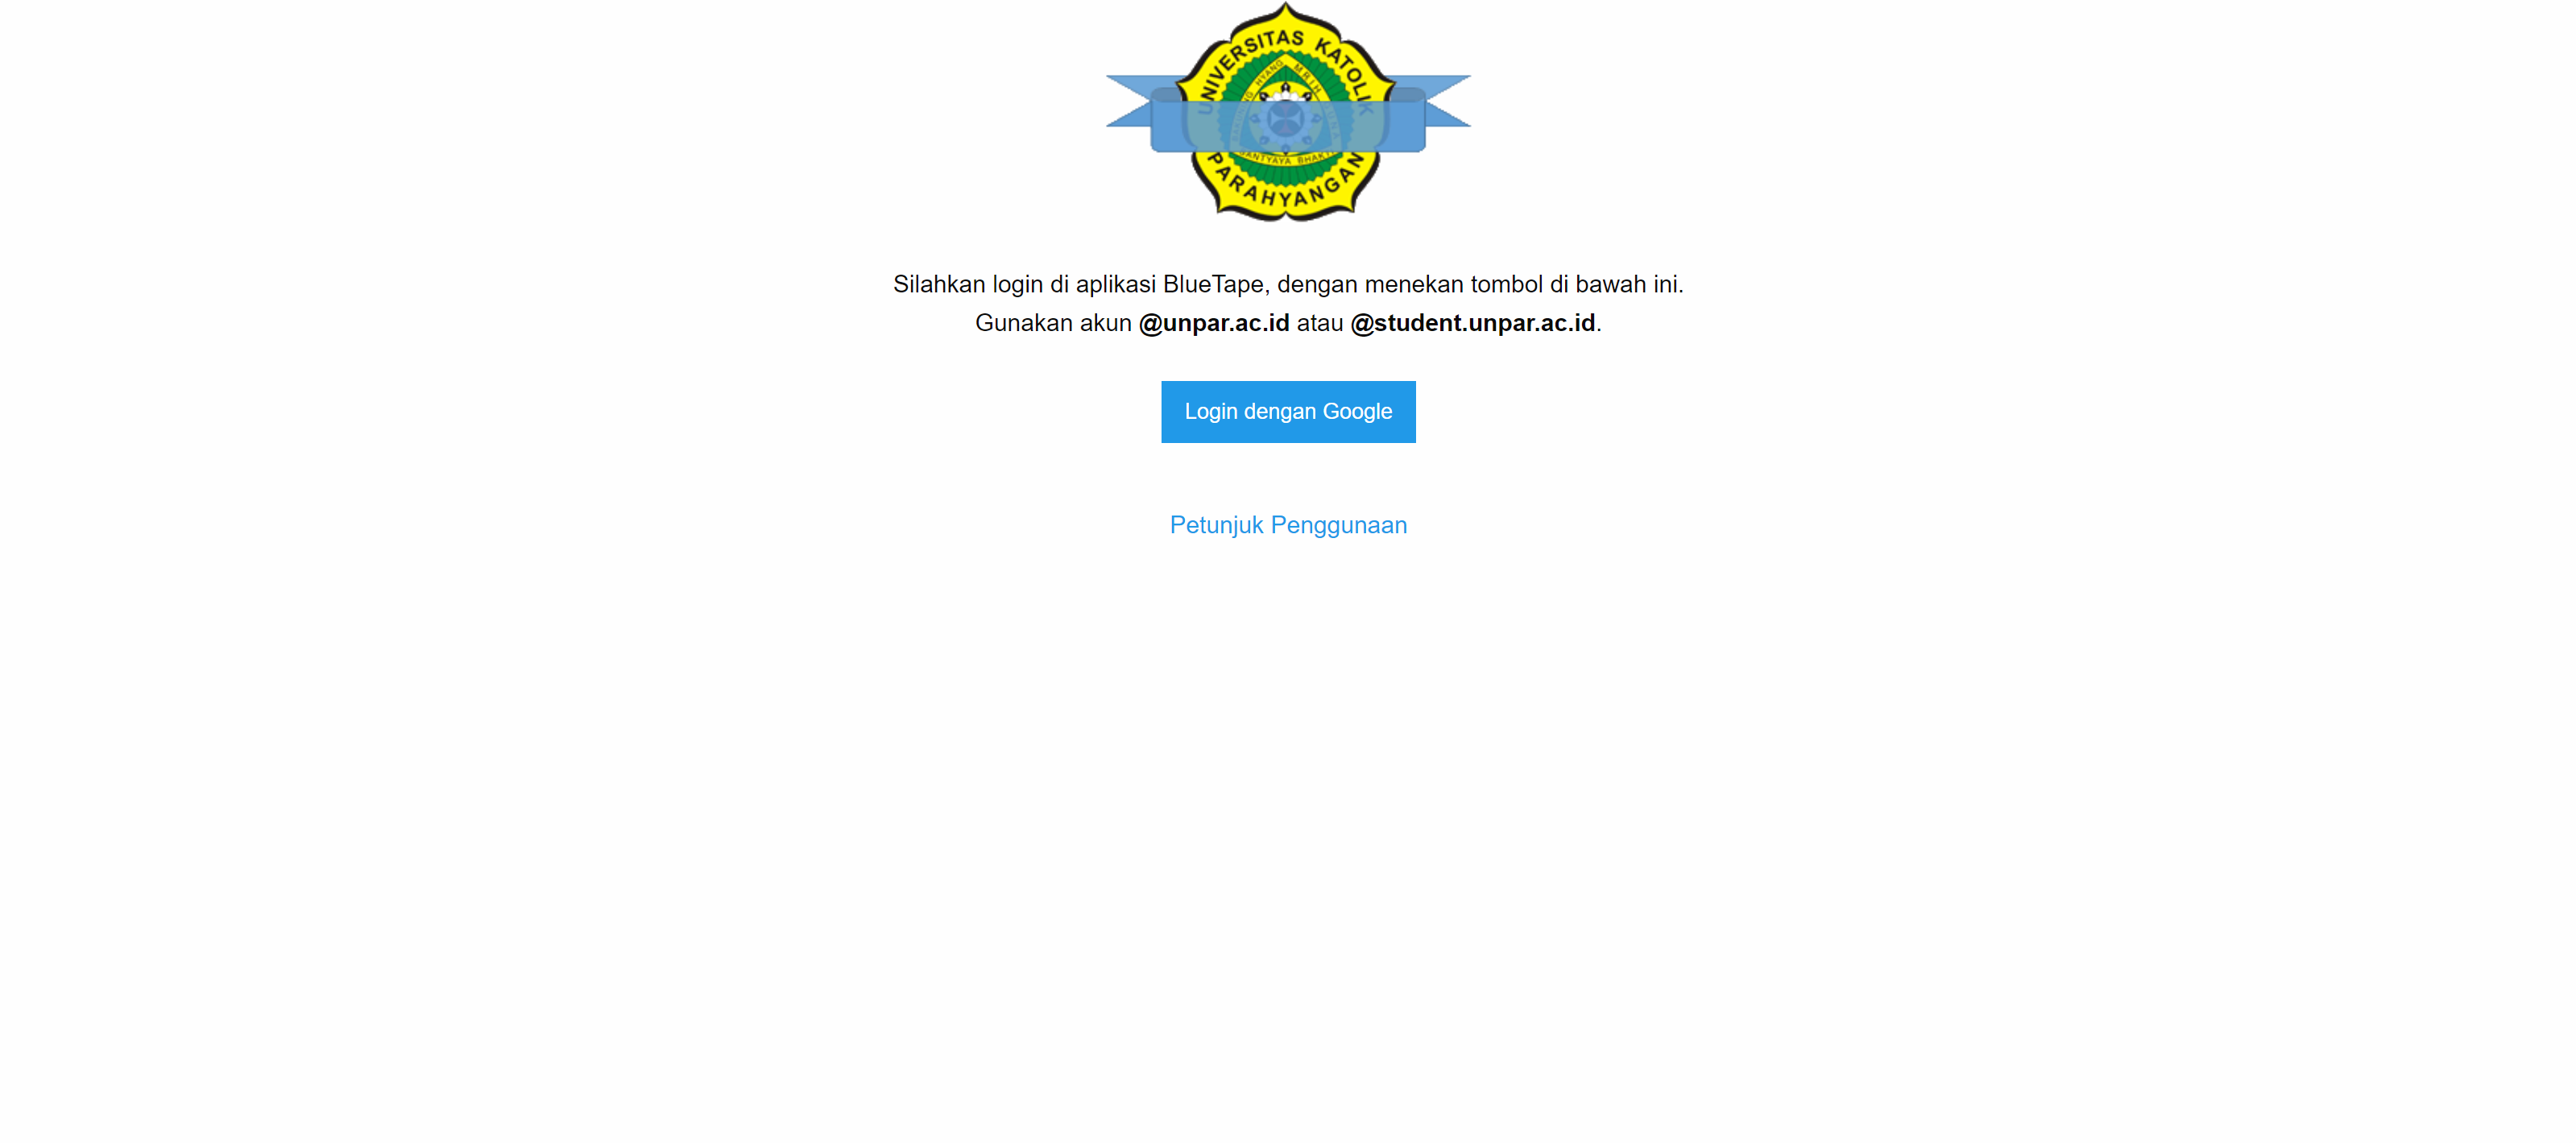
\includegraphics[scale=0.5]{Tampilan-Login.png}  
	\caption{Antarmuka Login BlueTape} 
\end{figure}
\noindent Antarmuka login tersimpan di folder \verb|auth| yang berisi tampilan HTML dan inisiasi file yang digunakan pada halaman ini. File css bootstrap akan didefinisikan disini. Analisis setiap bagian tampilan sebagai berikut :
\begin{itemize}
	\item Seluruh bagian disimpan dalam satu baris vertikal yang berukuran 6 grid. Sehingga dibutuhkan kelas \verb|row| \verb|col-lg-6| 	
	\item Text, logo dan link akan diletakkan ditengah, dibutuhkan kelas \verb|text-center|
	\item Tombol memiliki warna biru sehingga dibutuhkan kelas \verb|btn btn-primary|
\end{itemize}

\subsection{Antarmuka Cetak Transkrip}
Isi dari halaman antarmuka cetak transkrip terdiri dari dua bagian yaitu :
\begin{enumerate}
	\item \verb|Permohonan Baru| : Sistem akan memberikan dua tampilan untuk bagian ini, dengan kondisi sebagai berikut:
	\begin{itemize}
		\item Sistem akan menampilkan form pengajuan transkrip, apabila mahasiswa belum pernah mengajukan permohonan atau pengajuan sebelumnya  dikonfirmasi staf TU, maka mahasiswa dapat mengajukan permohonan baru.
		\item Sistem akan menampilkan informasi "Anda tidak bisa meminta cetak karena ada permintaan lain yang belum selesai", apabila mahasiswa memiliki pengajuan permohonan transkrip yang belum dikonfirmasi staf TU. 
	\end{itemize}
	\item \verb|Histori Permohonan| : Tabel untuk menampilkan informasi permohonan transkrip seorang mahasiswa. Status, tanggal pembuatan, tipe transkrip, tanggal cetak keterangan dan aksi. 
\end{enumerate}
Desain antarmuka sebagai berikut : \par
"Konten Permohonan Baru dan Histori permohonan" akan diletakkan pada sebuah \textit{container}, yang tiap konten nya akan dipisahkan oleh border yang memiliki padding. Sehingga dibutuhkan kelas \verb|container|, \verb|row|, \verb|col| dan \verb|p-*|. \par
Untuk konten Permohonan Baru :
\begin{itemize}
	\item Bagian isi akan memiliki dua tampilan yaitu berbentuk form atau notifikasi yang berbentuk paragraf. Sehingga dibutuhkan kelas \verb|form-control| dan \verb|<p>|.
	\item Untuk field pada baris pertama akan memiliki kolom dengan panjang 4 grid. Sehingga dibutuhkan kelas \verb|col-lg-4|.
	\item Untuk field pada baris kedua memiliki dua jenis lebar grid yaitu 4 grid dan 8 grid. Sehingga membutuhkan kelas \verb|col-lg-4|, \verb|col-lg-8|.
	\item Tombol "Kirim Permohonan" memiliki \textit{background color} berwarna biru sehingga akan digunakan kelas \verb|btn btn-primary|
\end{itemize}
Untuk konten Histori Permohonan :
\begin{enumerate}
	\item Terdapat sebuah tabel yang memiliki \verb|th| bersifat \textit{bold} sehingga dibutuhkan kelas \verb|table-active|. \verb|tbody| yang memiliki desain tabel bergaris sehingga dibutuhkan kelas \verb|table table-striped|.
	\item Pada kolom "Status" akan memiliki tiga jenis bentuk alert dengan \textit{backgroud} warna hijau, abu-abu dan merah. Sehingga dibutuhkan kelas \verb|bg-secondary|, \verb|bg-success|, \verb|bg-danger|.
	\item Aksi memiliki satu ikon "lihat" berwarna biru yang akan menampilkan sebuah modal. Sehingga dibutuhkan kelas ikon \verb|fas fa-eye|.
\end{enumerate}
\begin{figure} [H]
	\centering  
	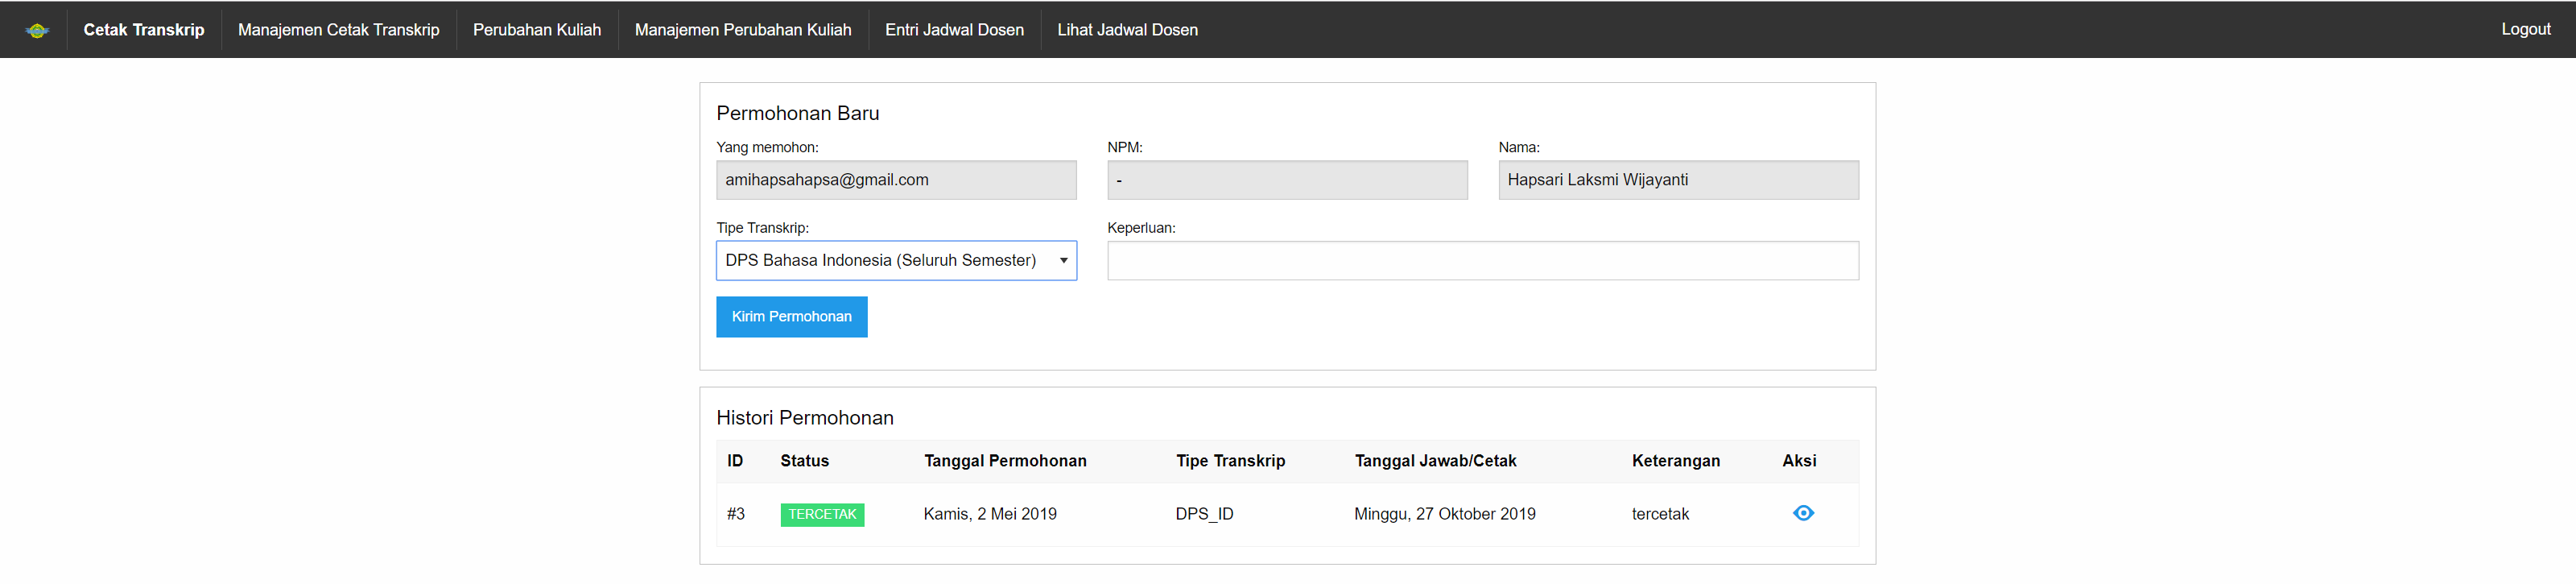
\includegraphics[scale=0.5]{Tampilan-Mahasiswa-Cetak-Transkrip.png}  
	\caption{Antarmuka Cetak Transkrip bagian 1} 
\end{figure}
\begin{figure} [H]
	\centering  
	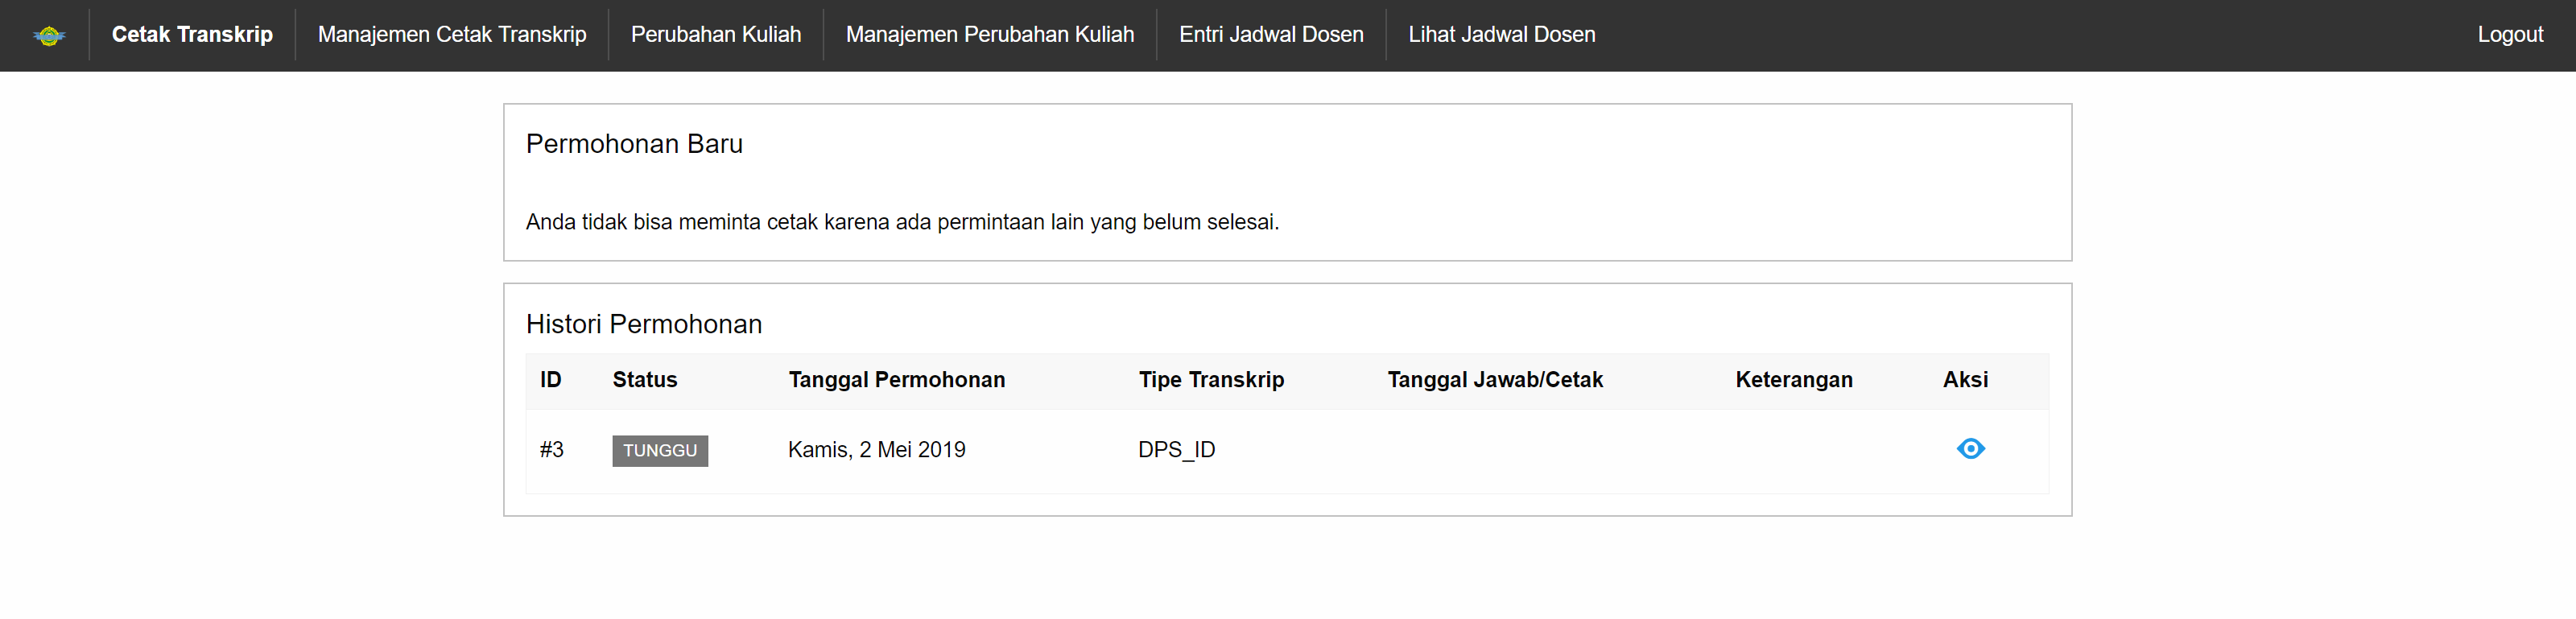
\includegraphics[scale=0.5]{Tampilan-Cetak-Transkrip.png}  
	\caption{Antarmuka Cetak Transkrip bagian 2} 
\end{figure}
Detail dari tabel permohonan baru, semua field akan  :
\begin{itemize}
	\item \texttt{Yang memohon} : Berisi email UNPAR mahasiswa, otomatis terisi saat login melalui gmail. Sehingga field tidak bisa diisi atau \textit{disabled} dibutuhkan atribut boolean \verb|readonly|
	\item \texttt{NPM} : Berisi NPM mahasiswa yang ter-\textit{generate} secara otomatis. Sehingga field tidak bisa diisi atau \textit{disabled} dibutuhkan atribut boolean \verb|readonly|
	\item \texttt{Nama} : Nama mahasiswa yang tergenerate secara otomatis. Sehingga field tidak bisa diisi atau \textit{disabled} dibutuhkan atribut boolean \verb|readonly|
	\item \texttt{Tipe Transkrip} : Terdiri dari tiga pilihan yaitu DPS Bahasa Indonesia(Seluruh Semester), DPS Bahasa Inggris(Seluruh Semester), LHS (Semester Terakhir). Wajib diisi.
	\item Keperluan : Keterangan keperluan dibuat nya transkrip, wajib diisi mahasiswa.
\end{itemize}
Apabila ada form yang belum diisi maka akan terdapat \textit{warning} untuk \textit{field} yang kosong.
Berikut ini apabila mahasiswa menekan tombol aksi lihat 
\includegraphics[height=0.7\baselineskip]{tombol_eye.png} :
\begin{figure} [H]
	\centering  
	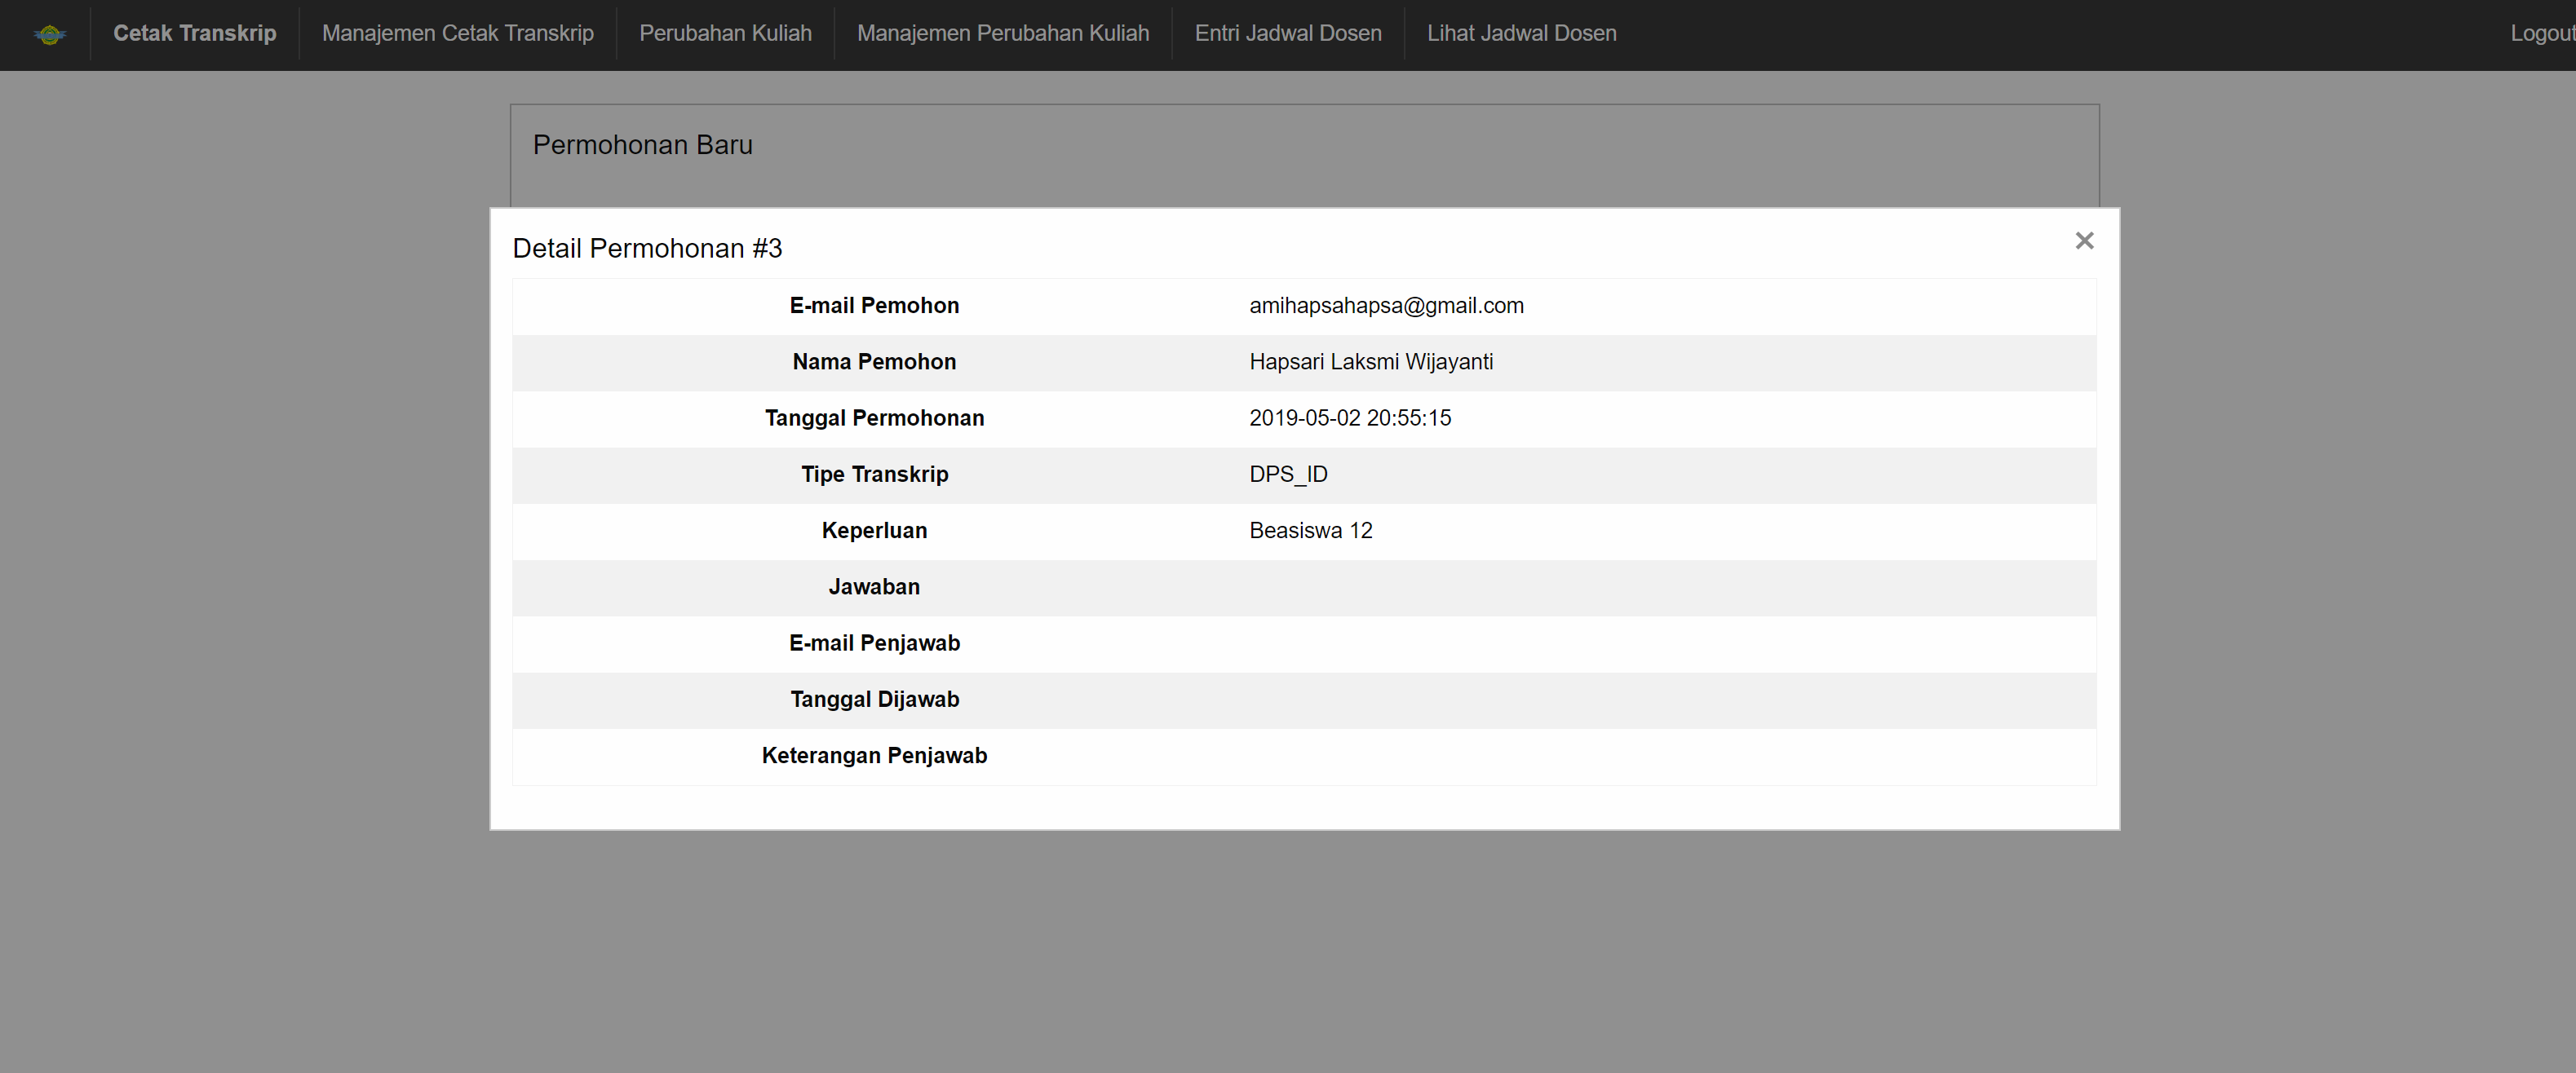
\includegraphics[scale=0.5]{Modal-Lihat-Cetak-Transkrip.png}  
	\caption{Modal Lihat Cetak Transkrip} 
\end{figure}
\noindent Disini aksi 'lihat' akan menampilkan sebuah modal yang berisi sebuah tabel bergaris yang menyimpan informasi detil permohonan, baik detil informasi dari mahasiswa maupun konfirmasi dari staf Tata Usaha. Sehingga dibutuhkan kelas \verb|modal-fade| dan \verb|table table-stripped|.

\subsection{Antarmuka Manajemen Cetak Transkrip}
\begin{figure} [H]
	\centering  
	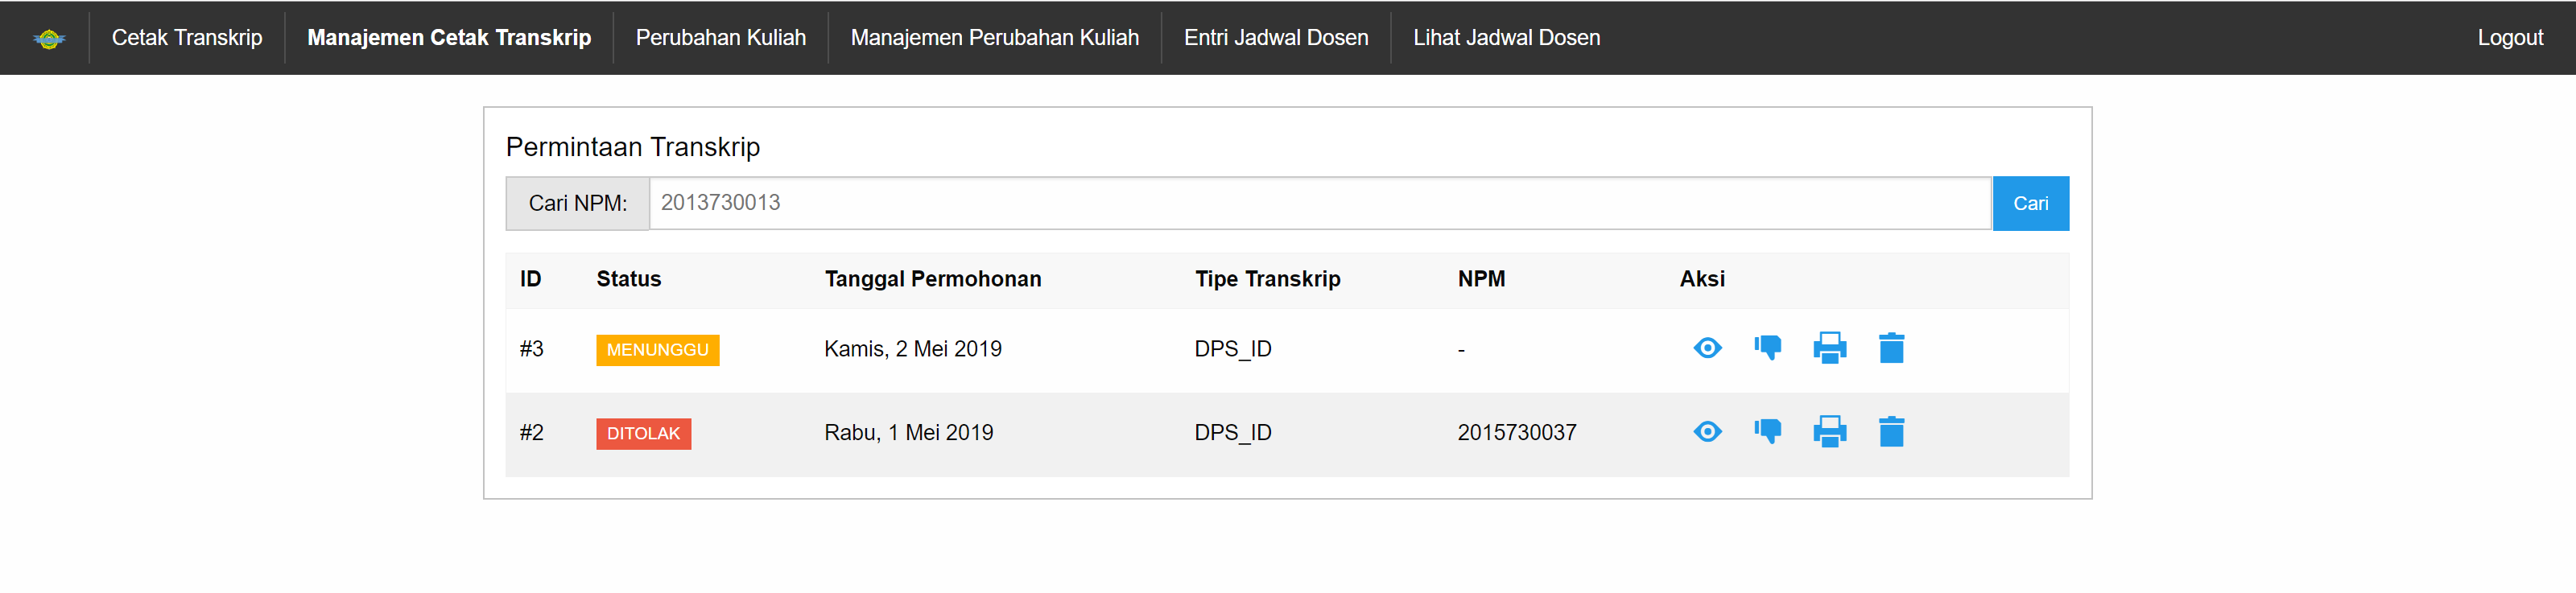
\includegraphics[scale=0.5]{Tampilan-Manajemen-Cetak-Transkrip.png}  
	\caption{Tampilan Manajemen Cetak Transkrip} 	
\end{figure}

Tampilan Manajemen Cetak Transkrip berisi sebuah tabel permintaan transkrip yang terdiri dari daftar permintaan transkrip dan form pencarian transkrip berdasarkan NPM. \par

\noindent Detail penjelasan untuk field 'Status' dan 'Aksi' :
\begin{itemize}
	\item[ ] \texttt{Status} : Output terdiri dari tiga jenis label yaitu 'MENUNGGU'(berwarna kuning), 'DITOLAK' (berwarna merah) dan 'TERCETAK'(berwarna hijau).  Sehingga dibutuhkan kelas \verb|bg-secondary|, \verb|bg-success|, \verb|bg-danger|. 
	\item[ ] \texttt{Aksi} : Terdiri dari empat ikon font-awesome yaitu \verb|fas fa-eye, fas fa-eye,fas fa-eye,fas fa-eye,| yang akan menampilkan modal berisi informasi yang sesuai dengan perintah.
\end{itemize}
Detail penjelasan untuk modal :
\begin{enumerate}
	\item Modal Lihat : Terdiri dari sebuah tabel bergaris sehingga membutuhkan kelas \verb|table table-striped|.
	\item Modal Tolak : Terdiri dari sebuah form yang terdiri dari label, field dan tombol berwarna merah yang diletakan dalam satu baris yang memanjang secara vertikal sehingga membutuhkan kelas \verb|col-form-label, form-control, row, col-lg-*, btn btn-danger|.
	\item Modal Print : Terdiri dari sebuah form yang terdiri dari label, field dan tombol berwarna merah yang diletakan dalam satu baris yang memanjang secara vertikal sehingga membutuhkan kelas \verb|col-form-label, form-control, row, col-lg-*, btn btn-primary|.
	\item Modal Hapus : Terdiri dari sebuah form yang terdiri dari paragraf yang bersifat bold dan tombol berwarna merah yang diletakan dalam satu baris yang memanjang secara vertikal sehingga membutuhkan kelas \verb|<p>, row, btn btn-danger|.
\end{enumerate}

\begin{figure} [H]
	\centering  
	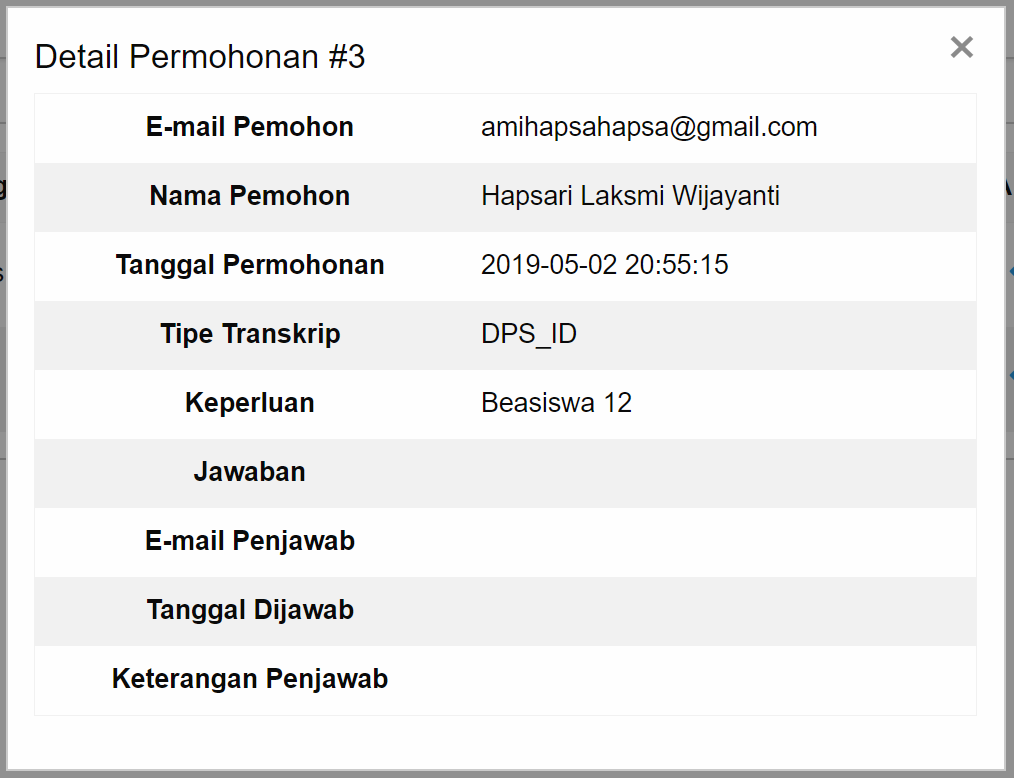
\includegraphics[scale=0.5]{Modal-Lihat-Manajemen-Cetak-Transkrip.png}  
	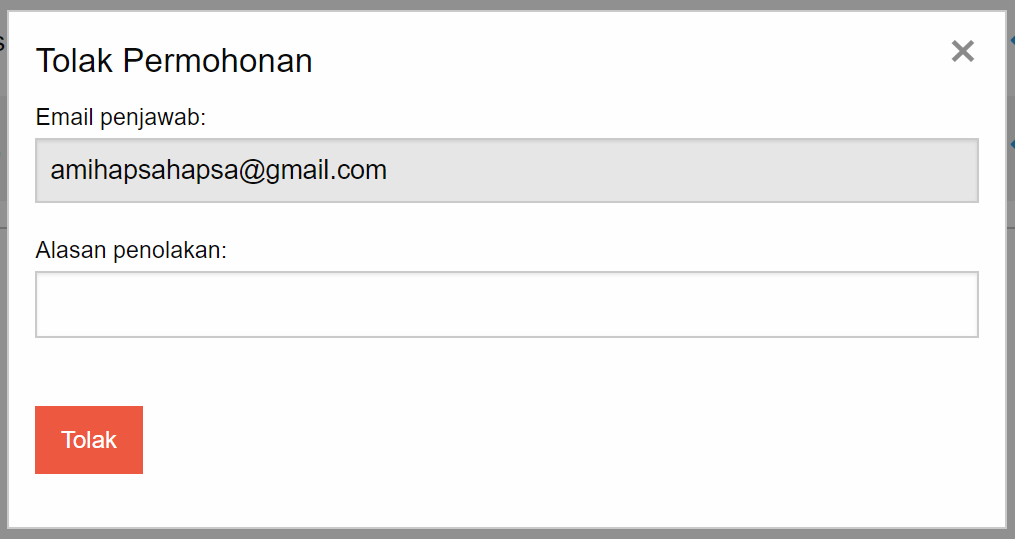
\includegraphics[scale=0.5]{Modal-Tolak-Manajemen-Cetak-Transkrip.png} 
	\caption{Tampilan Modal untuk aksi 'Lihat' dan 'Tolak'} 	
\end{figure}

\begin{figure} [H]
	\centering  
	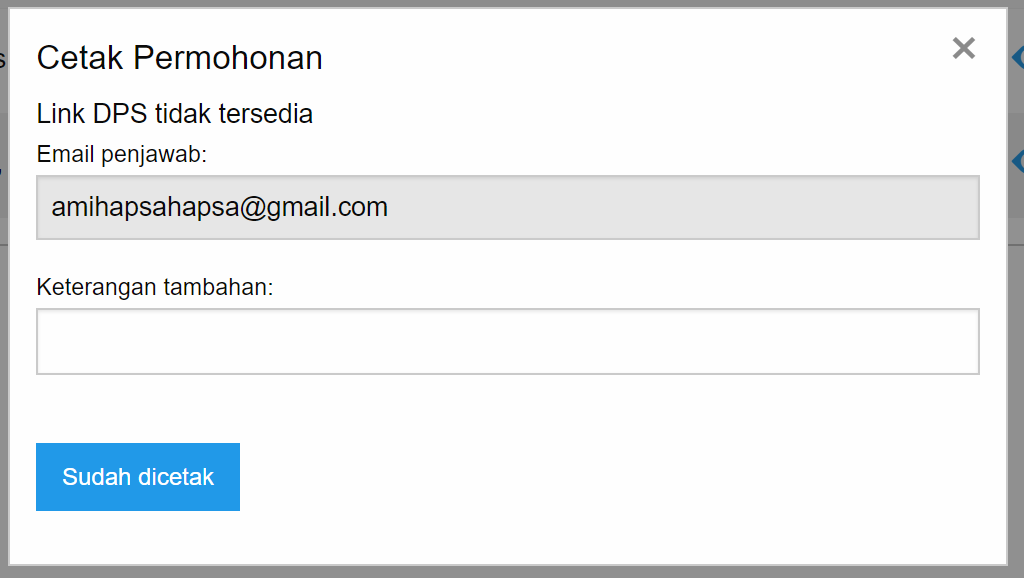
\includegraphics[scale=0.5]{Modal-Print-Manajemen-Cetak-Transkrip.png}  
	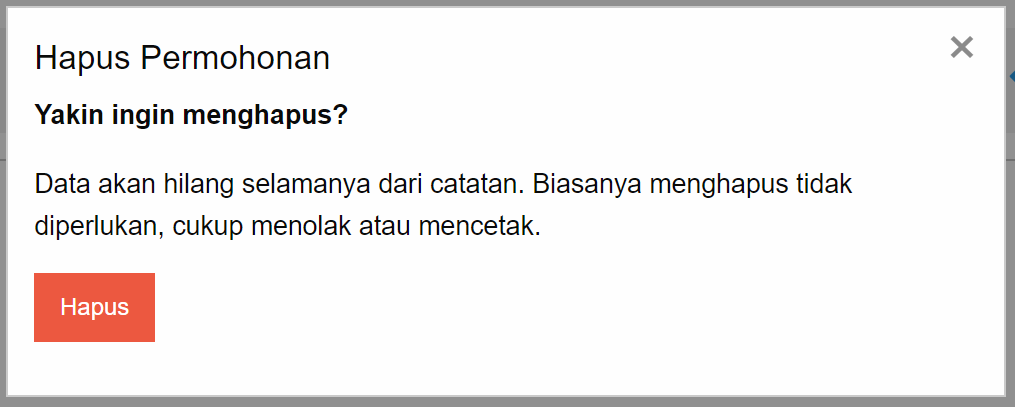
\includegraphics[scale=0.5]{Modal-Hapus-Manajemen-Cetak-Transkrip.png} 
	\caption{Tampilan Modal untuk aksi 'Print' dan 'Hapus'} 	
\end{figure}


\subsection{Antarmuka Perubahan Kuliah}
\begin{figure} [H]
	\centering  
	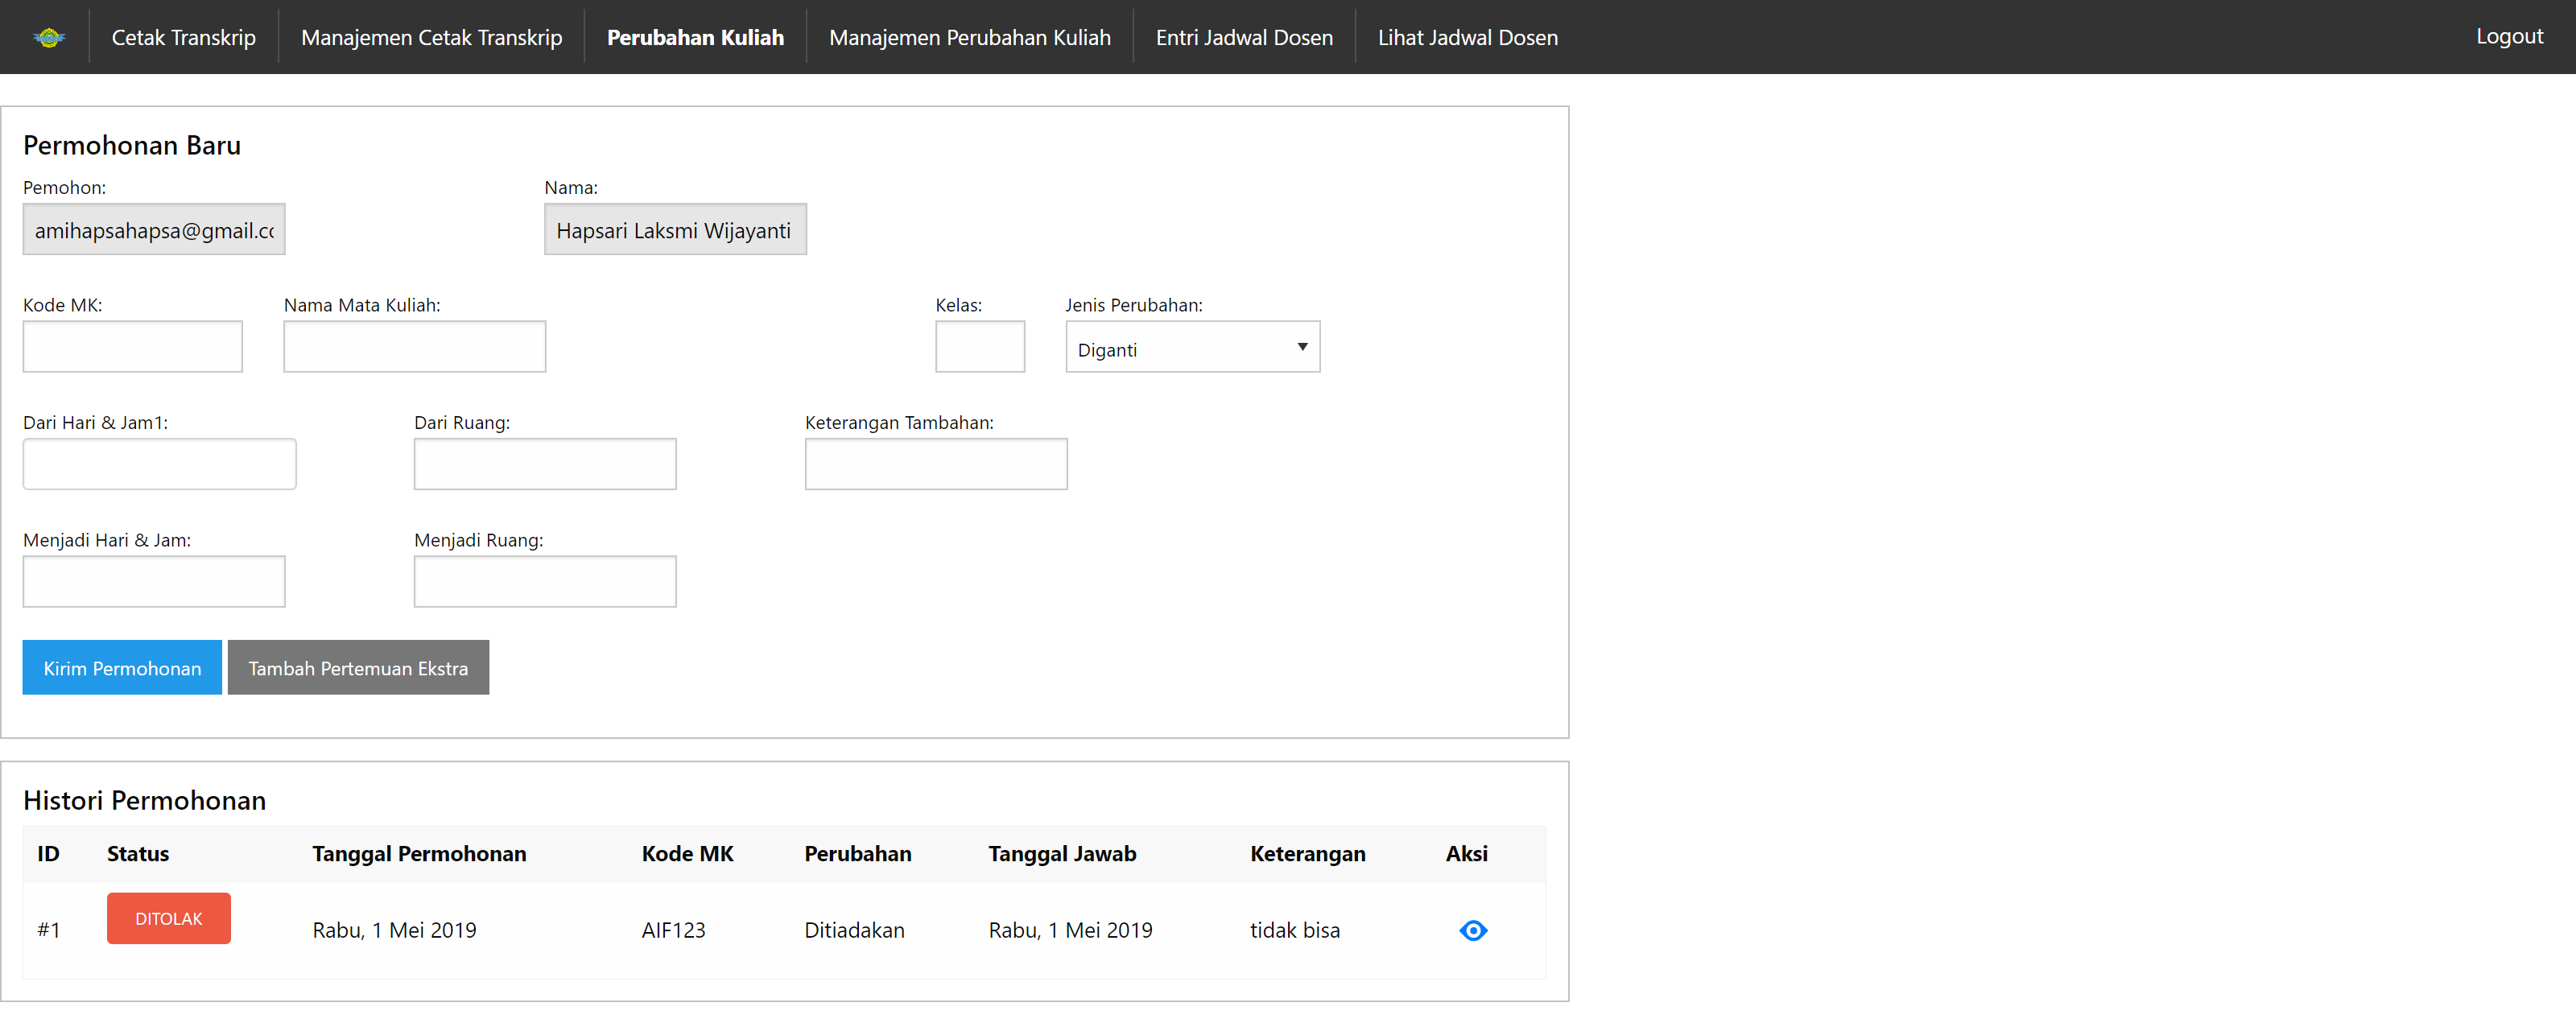
\includegraphics[scale=0.5]{Tampilan-Perubahan-Kuliah.png}  
	\caption{Tampilan Perubahan Kuliah} 
\end{figure}
Modul Perubahan Kuliah terdiri dari dua tabel yaitu :

\subsection{Permohonan Baru}

\begin{tabular}{ |p{4cm}|p{2cm}|p{10cm}|}
	\hline
	Nama Kolom & Pilihan & Keterangan\\
	\hline
	\texttt{Pemohon} &  &Field terisi secara otomatis, user tidak bisa mengisi field atau \textit{disabled} dan memiliki lebar 4 grid, sehingga membutuhkan kelas \verb|readonly, col-lg-4, form-control|.\\
	\hline
	\texttt{Nama} &  & Field terisi secara otomatis, user tidak bisa mengisi field atau \textit{disabled} dan memiliki lebar 4 grid, sehingga membutuhkan kelas \verb|readonly, col-lg-8, form-control|.\\
	\hline
	\texttt{Kode MK} & & Field bertipe text dan memiliki lebar 2 grid , sehingga membutuhkan kelas \verb|col-lg-2, form-control|.\\
	\hline
	\texttt{Nama Mata Kuliah} & & Field bertipe text dan memiliki lebar 5 grid, sehingga membutuhkan kelas \verb|form-control, col-lg-5| \\
	\hline
	\texttt{Kelas} &  & Field bertipe text dan memiliki lebar 1 grid, sehingga membutuhkan kelas \verb|form-control, col-lg-1| \\
	\hline
	\texttt{Jenis Perubahan} & Diganti &  Field 'Dari Hari dan Jam' dan 'Dari Ruang' disabled  \\
	& Tambahkan &    Field 'Dari Hari dan Jam' dan 'Dari Ruang' dapat ditambahkan lebih dari satu kolom dan memiliki lebar 4 grid, sehingga membutuhkan kelas \verb|form-control, col-lg-4|\\	 
	& Ditiadakan &  Field 'Menjadi Hari dan Jam' dan 'Menjadi Ruangan' disabled, sehingga membutuhkan kelas \verb|readonly|  \\
	\hline
	\texttt{Dari Hari dan Jam} &  & Menggunakan plugin bootstrap \textit{calendar} yang bisa menampilkan pilihan tanggal dan waktu \\
	\hline
	\texttt{Dari Ruang} &  & Field bertipe text, sehingga membutuhkan kelas \verb|form-control| \\
	\hline
	\texttt{Keterangan Tambahan} &  & Field bertipe text, sehingga membutuhkan kelas \verb|form-control| \\
	\hline
	\texttt{Menjadi Hari dan Jam} &  & Menggunakan plugin \textit{calendar} \\
	\hline
	\texttt{Menjadi Ruangan} &  & Field bertipe text, sehingga membutuhkan kelas \verb|form-control| \\
	\hline
\end{tabular}

\subsection{Histori Pemohonan}
\begin{tabular}{ |p{4cm}|p{2cm}|p{10cm}|  }
	\hline
	Nama Kolom & Pilihan & Keterangan\\
	\hline
	\texttt{Status} & dikonfirmasi, menggunakan kelas \verb|bg-success| & Apabila staf TU menyetujui permohonanan\\
	\hline
	&  ditolak, menggunakan kelas \verb|bg-danger|  & Apabila staf TU menolak permohonanan\\
	\hline
	& ditunggu, menggunakan kelas \verb|bg-secondary| &  Apabila staf TU belum konfirmasi permohonan \\
	\hline
	\texttt{Tanggal Permohonan}    & & Data bertipe tanggal yang sudah diconvert\\
	\hline
	\texttt{Kode MK} &  & Field bertipe text, menggunakan kelas \verb|form-control| \\
	\hline
	\texttt{Perubahan} &  &  Konfirmasi staf TU : Diganti, Ditambahkan, Ditiadakan, menggunakan \verb|select| yang menggunakan kelas \verb|form-control| \\
	\hline
	\texttt{Tanggal Jawab} &  & Data bertipe tanggal \\
	\hline
	\texttt{Keterangan} &  & Field bertipe text, menggunakan kelas \verb|form-control| \\
	\hline
	\texttt{Aksi} &  & Terdapat tombol aksi 'Lihat', menggunakan font awesome dan kelas \verb|fas fa-eyes| \\
	\hline
\end{tabular}
Ketika user menekan tombol aksi 'lihat', maka modal berisi informasi data permohonan yang sesuai dengan ID 
\begin{figure} [H]
	\centering  
	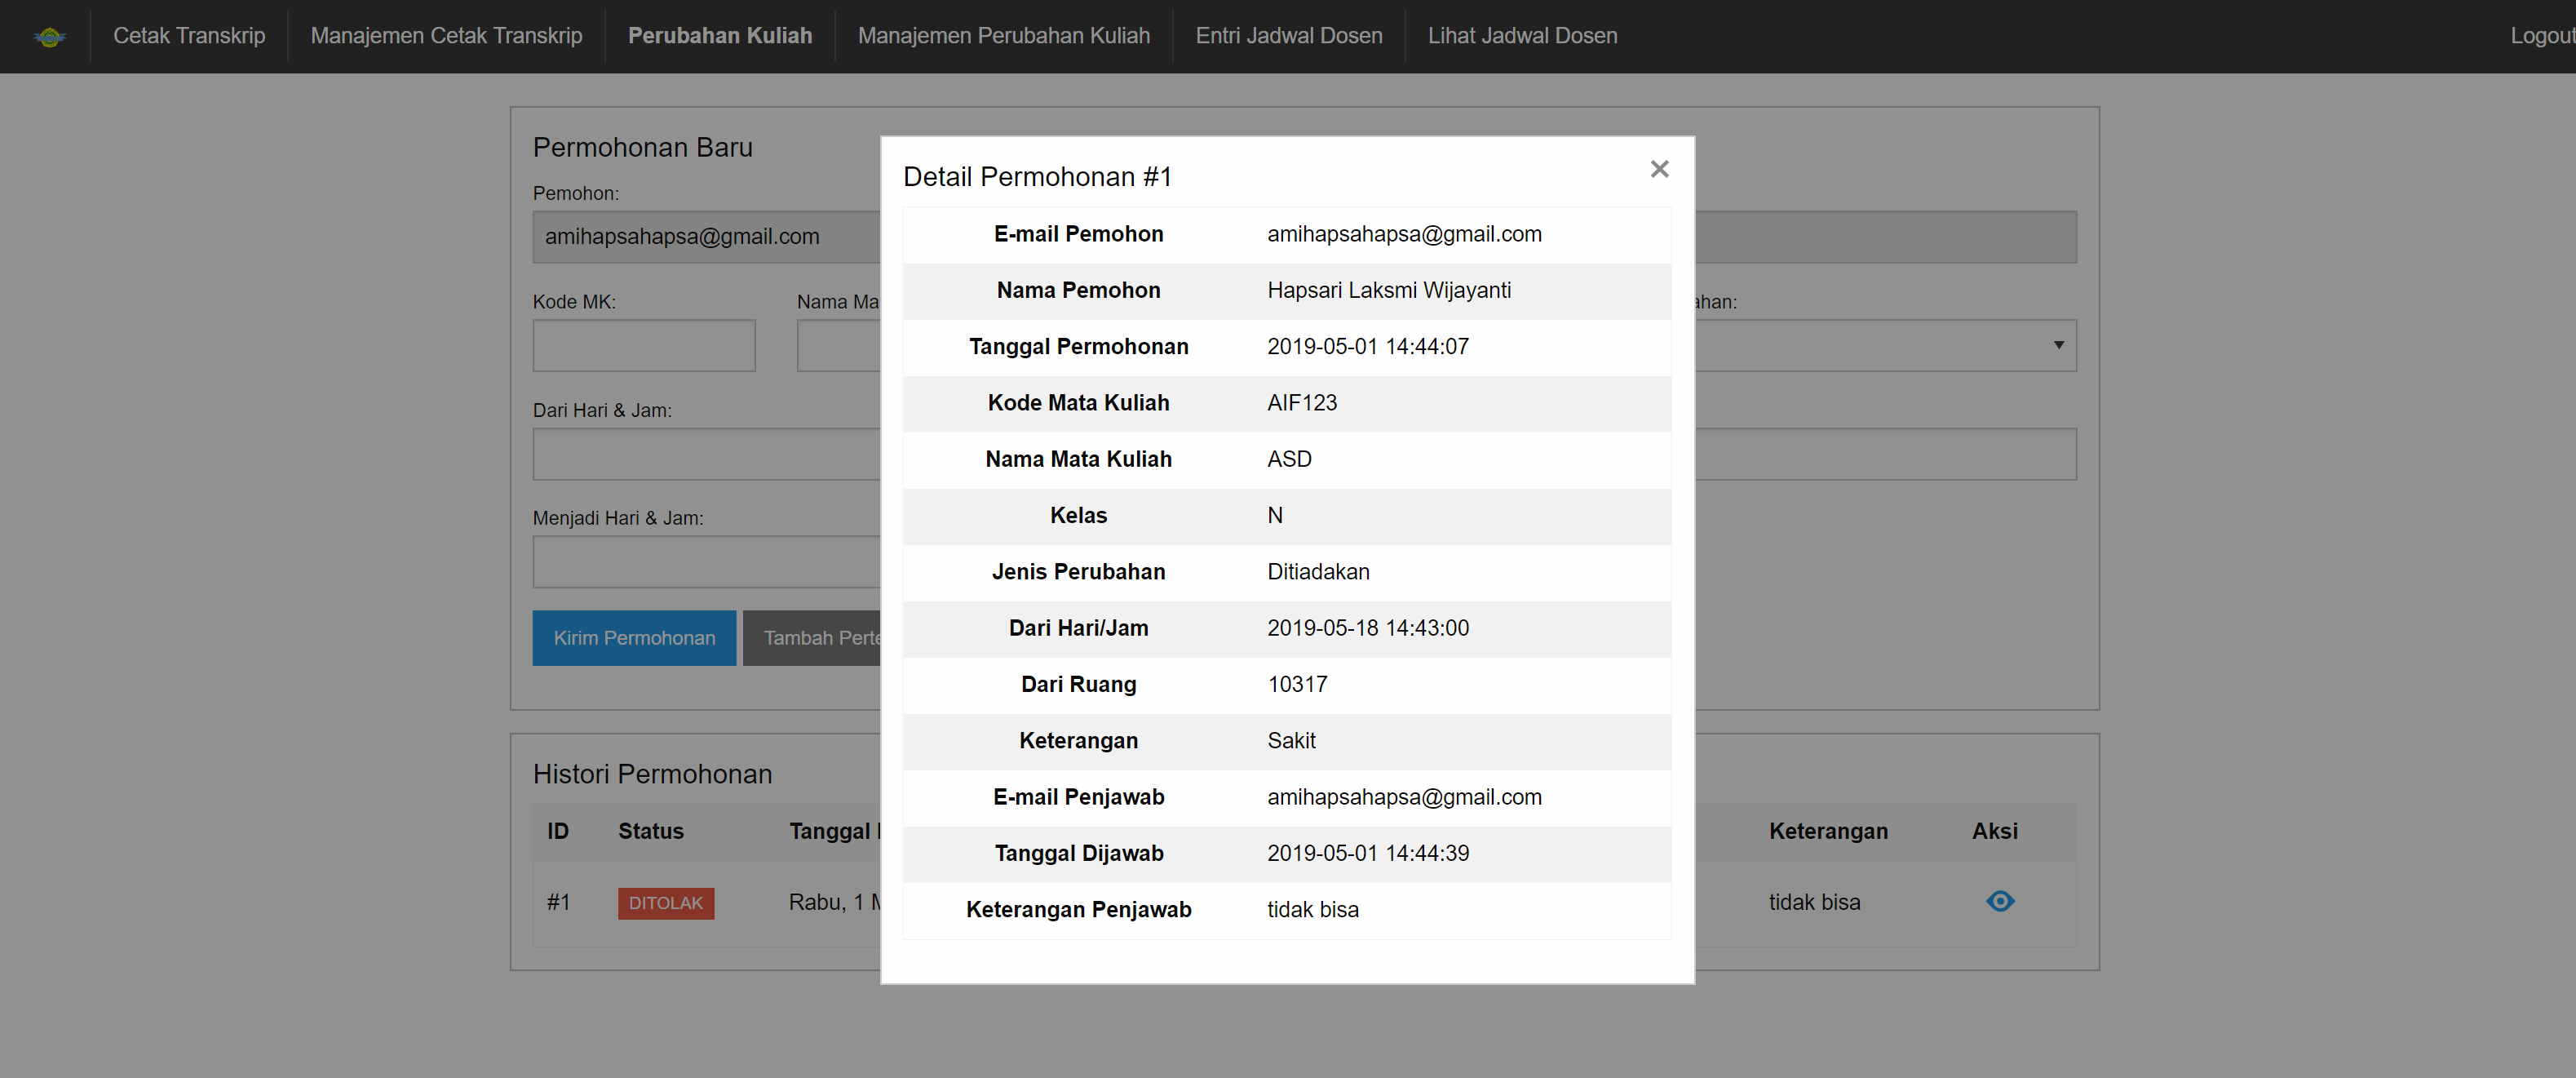
\includegraphics[scale=0.5]{Modal-Lihat-Perubahan-Kuliah.png}  
	\caption{Modal Lihat Perubahan Kuliah} 
\end{figure}


\subsection{Antarmuka Manajemen Perubahan Kuliah}
\begin{figure} [H]
	\centering  
	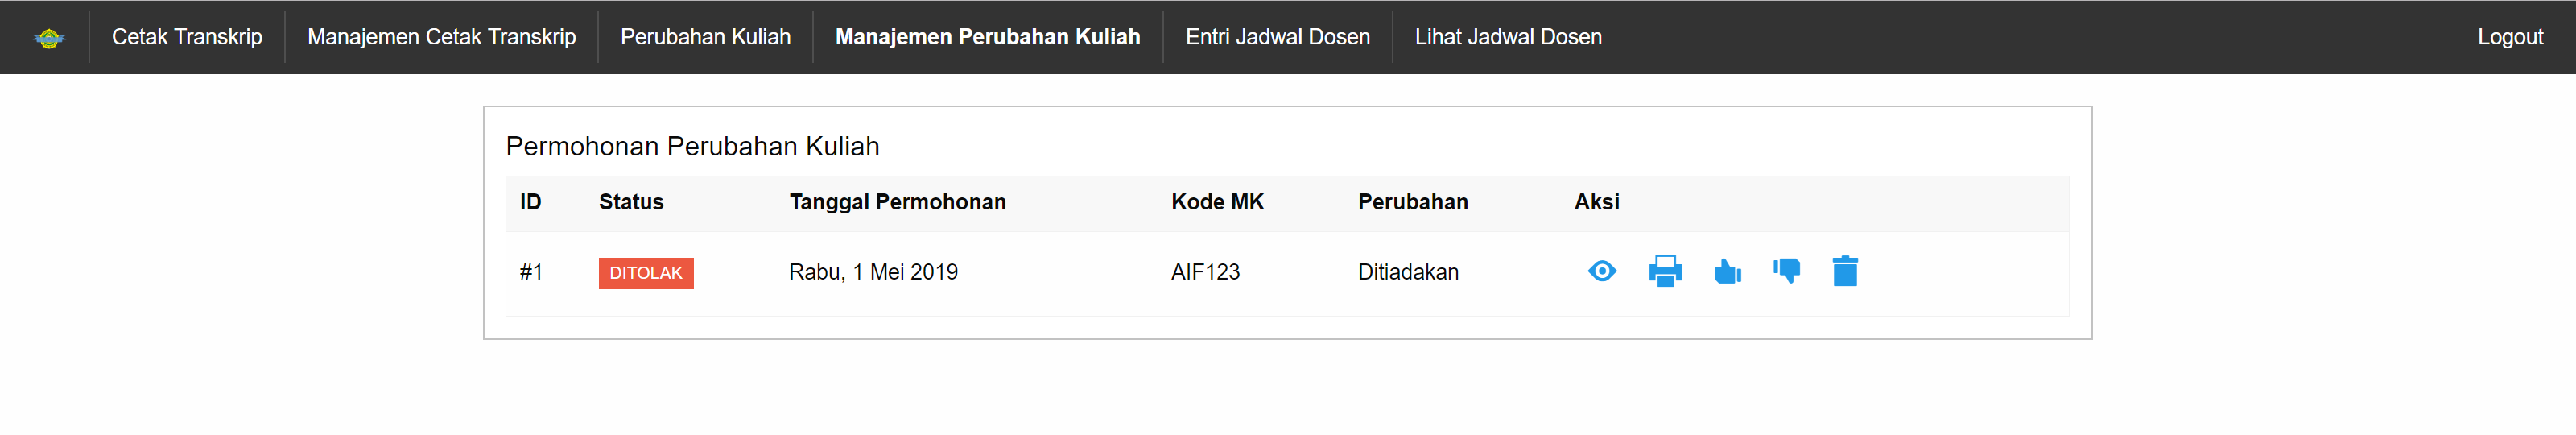
\includegraphics[scale=0.5]{Tampilan-Manajemen-Perubahan-Kuliah.png}  
	\caption{Tampilan Manajemen Perubahan Kuliah} 
\end{figure}
Tabel Pemohonan Kuliah memiliki detail yang sama dengan tabel histori permohonan, namun aksi yang dilakukan terdiri dari lima perintah:
\begin{figure} [H]
	\centering  
	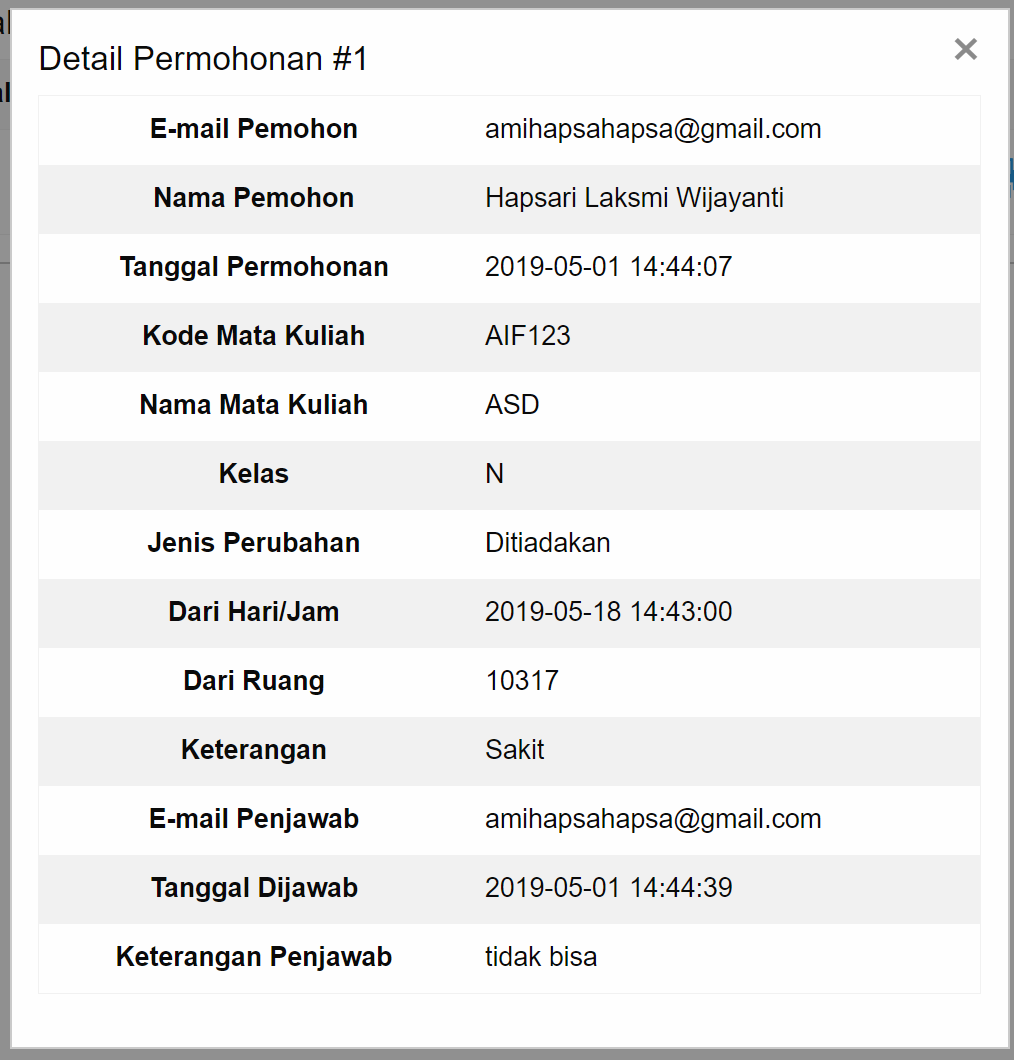
\includegraphics[scale=0.3]{Modal-Lihat-Manajemen-Perubahan-Kuliah.png}  
	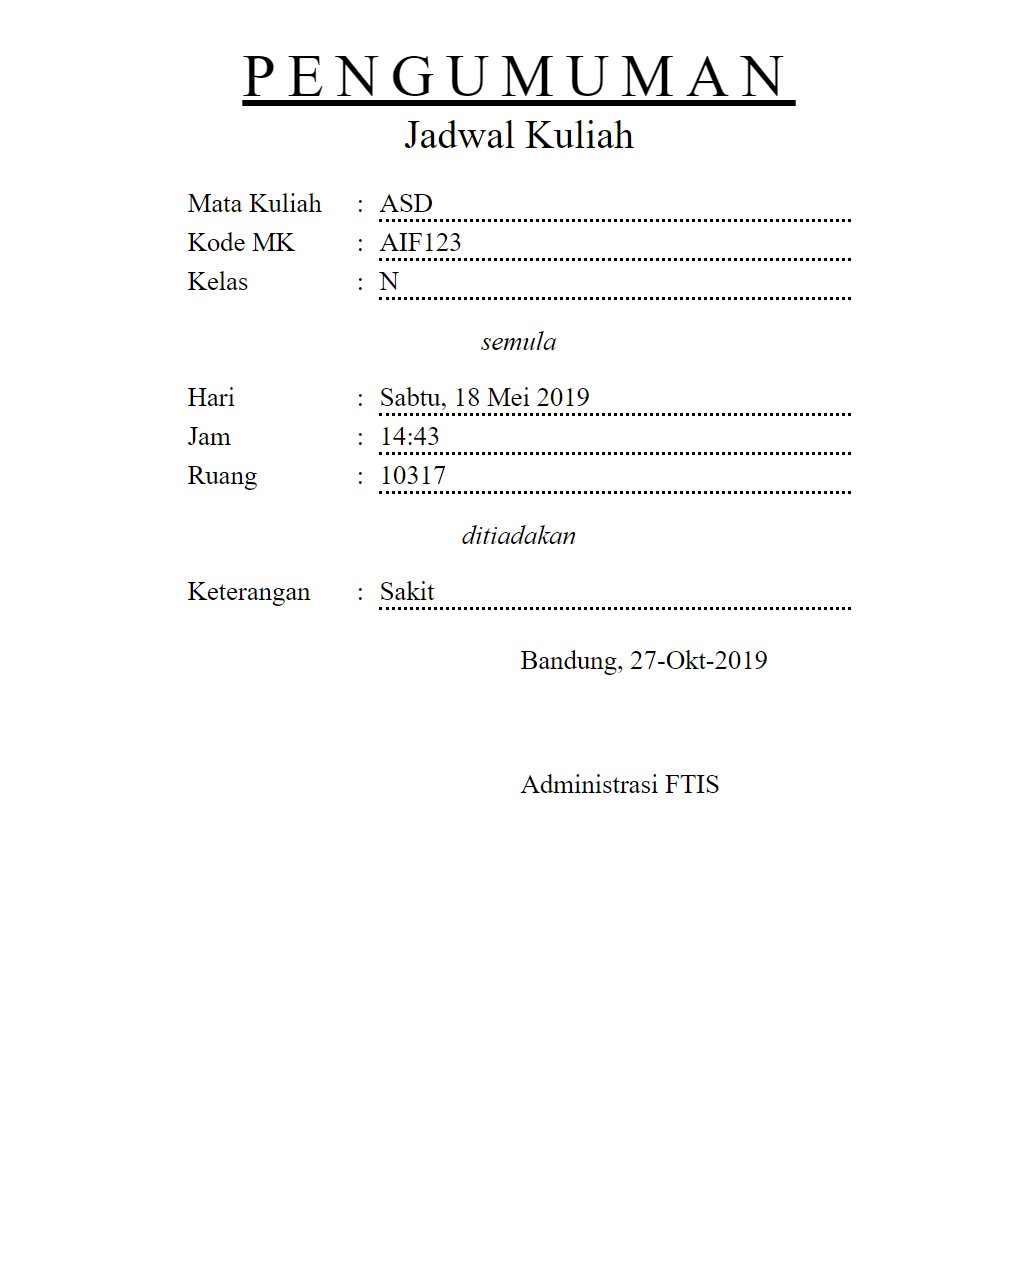
\includegraphics[scale=0.3]{Modal-Print-Manajemen-Perubahan-Kuliah.png} 
	\caption{Modal aksi Lihat dan Print Manajemen Perubahan Kuliah} 
\end{figure}
\begin{figure} [H]
	\centering  
	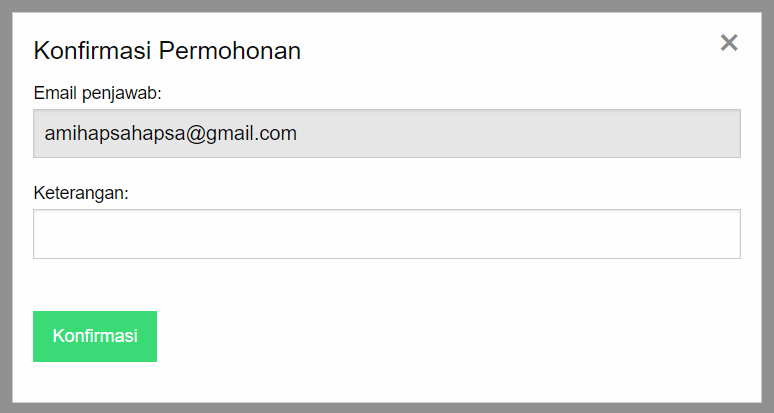
\includegraphics[scale=0.3]{Modal-Setuju-Manajemen-Perubahan-Kuliah.png}
	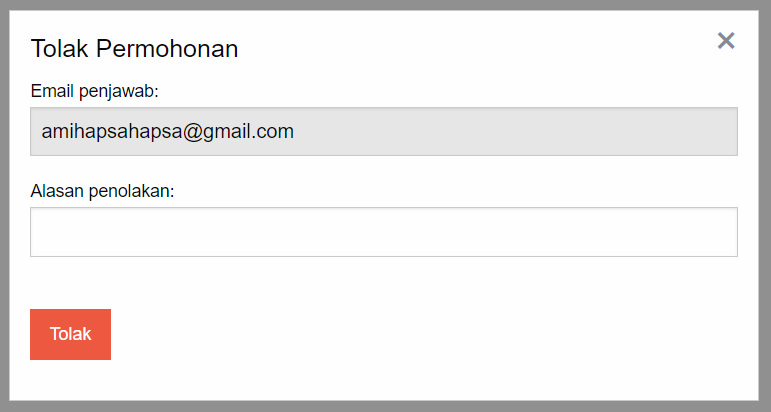
\includegraphics[scale=0.3]{Modal-Tolak-Manajemen-Perubahan-Kuliah.png}    
	\caption{Modal aksi Setuju dan Tolak Manajemen Perubahan Kuliah} 
\end{figure}
\begin{figure} [H]
	\centering  
	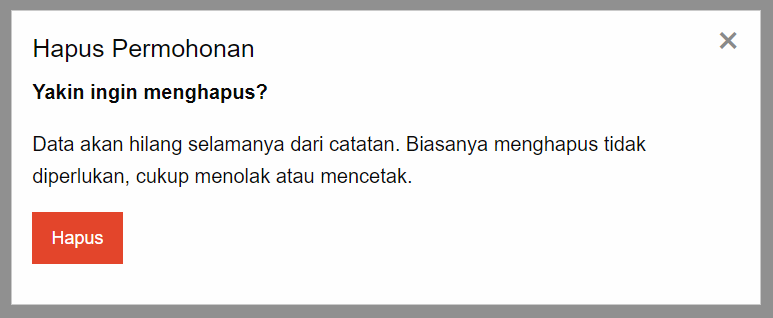
\includegraphics[scale=0.3]{Modal-Hapus-Manajemen-Perubahan-Kuliah.png}  
	\caption{Modal Hapus Manajemen Perubahan Kuliah} 
\end{figure}

\subsection{Antarmuka Entri Jadwal Dosen}
\begin{figure} [H]
	\centering  
	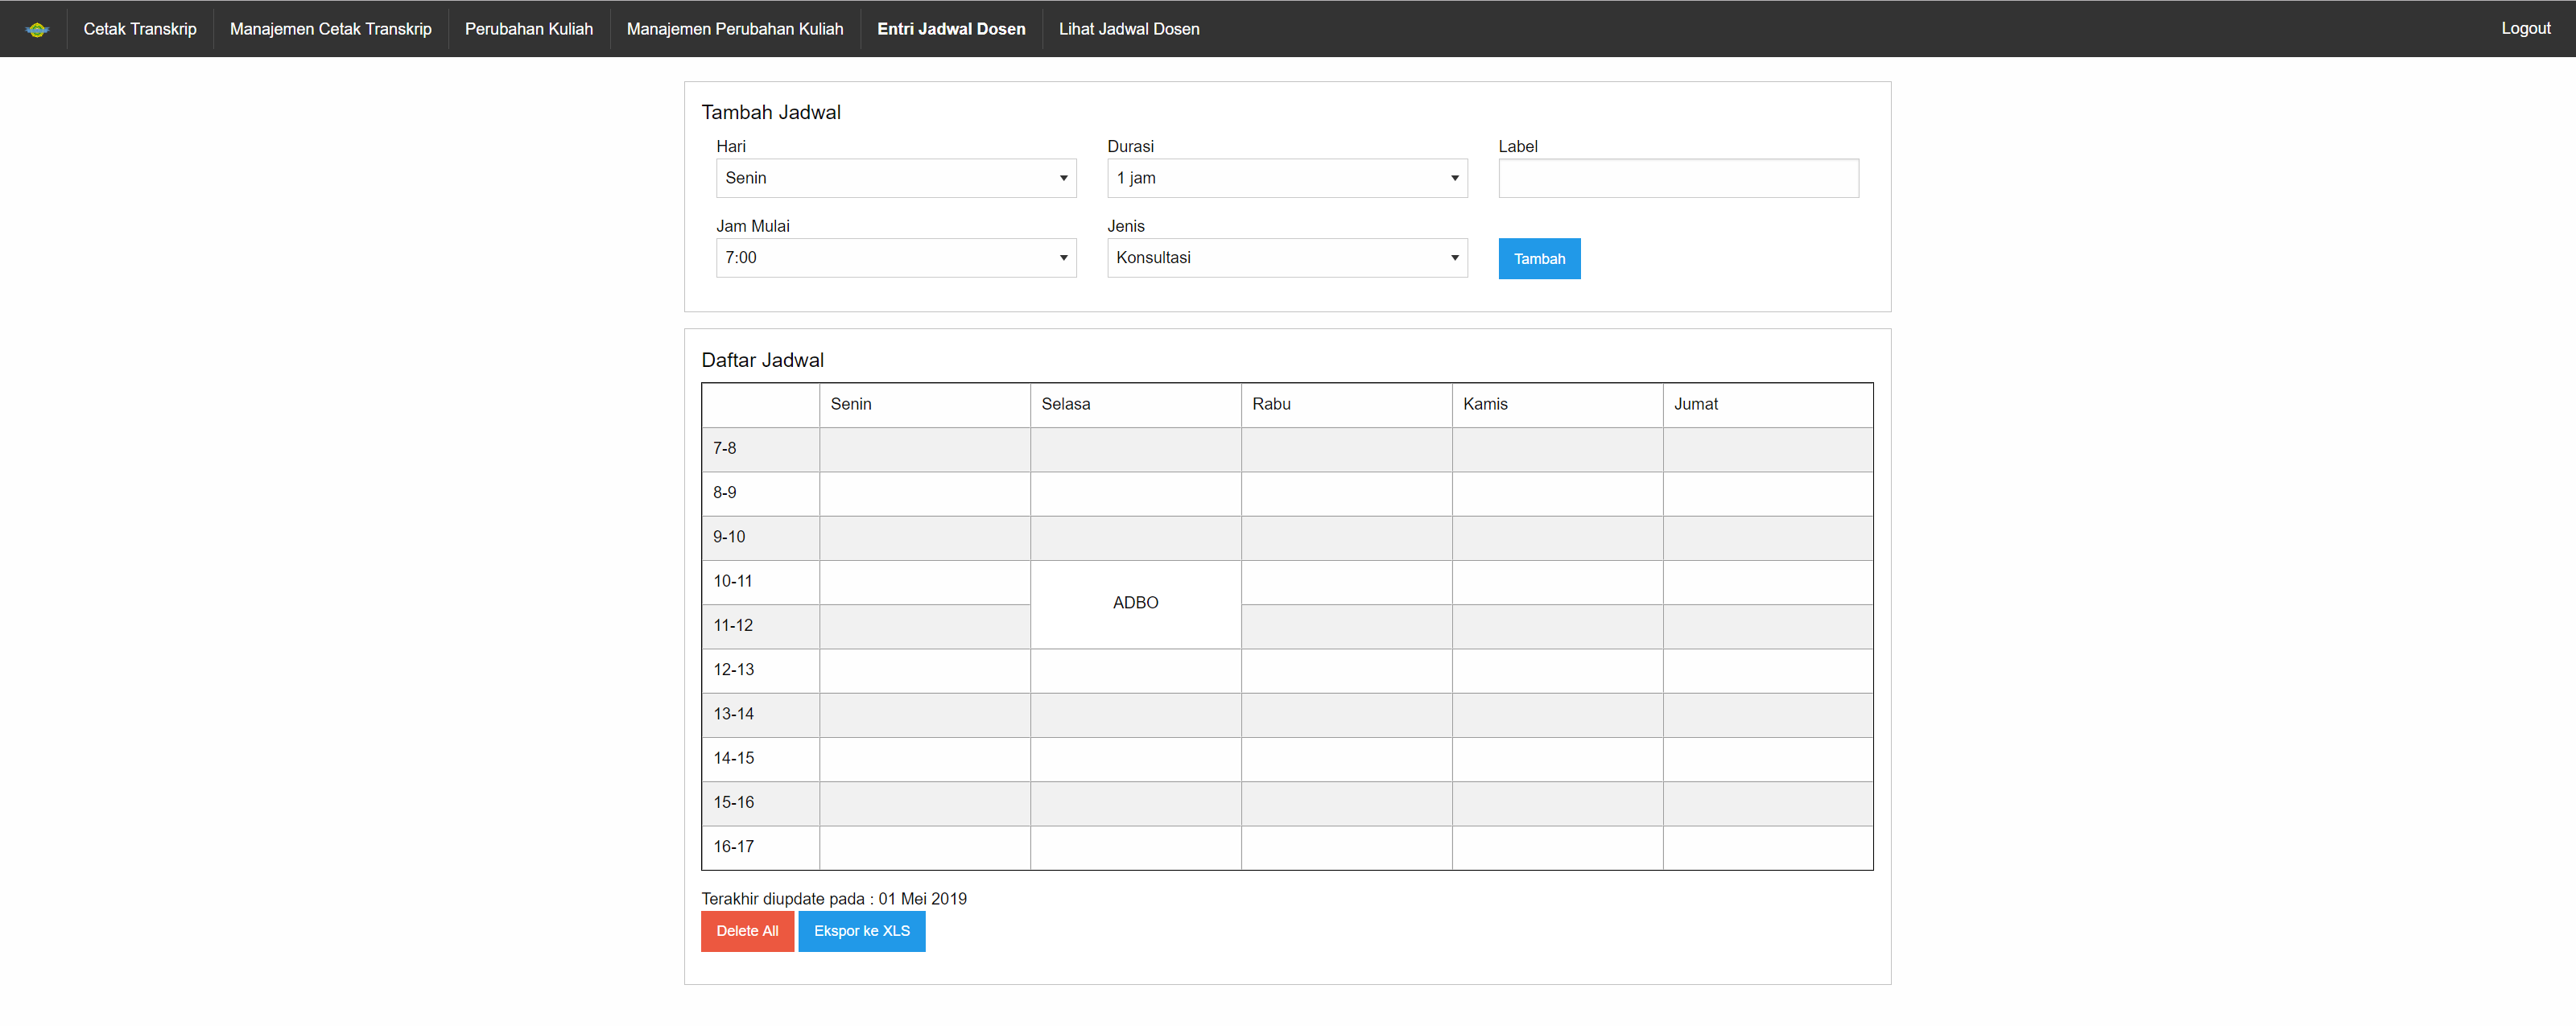
\includegraphics[scale=0.5]{Tampilan-Entri-Jadwal-Dosen.png}  
	\caption{Modal Print Manajemen Perubahan Kuliah} 
\end{figure}
Detail mengenai tabel Tambah Jadwal :
\begin{itemize}
	\item \texttt{Hari} : Terdiri dari nama hari dari senin sampai jumat.
	\item \texttt{Durasi} : Terdiri dari rentang jam kelas berlangsung dari 1 jam hingga 9 jam.
	\item \texttt{Label} : Field bertipe text.
	\item \texttt{Jam Mulai} : Terdiri dari jam dari rentang 07:00 sampai 16:00.
	\item \texttt{Jenis} : Terdiri dari tiga macam pilihan 
	\begin{enumerate}
		\item Konsultasi : Memiliki background berwarna hijau.
		\item Terjadwal : Memiliki background berwarna biru.
		\item Kelas : Memiliki background putih.
	\end{enumerate}
\end{itemize}

Tabel Daftar jadwal akan \textit{retrieve} data jadwal dari dosen yang dibuat. Terdiri dari rentang waktu dan hari. Jadwal yang terlihat pada tabel ini bisa diedit dan dihapus.
Dibagian bawah tabel akan terlihat tanggal jadwal tersebut di update dan memiliki dua tombol :
\begin{itemize}
	\item \texttt{Delete All} : Menghapus semua jadwal yang sudah dibuat.
	\item \texttt{Export ke XLS} : Secara otomatis akan membuat file excel dan mendownload di device secara lokal.
\end{itemize}

\subsection{Antarmuka Lihat Jadwal Dosen}
\begin{figure} [H]
	\centering  
	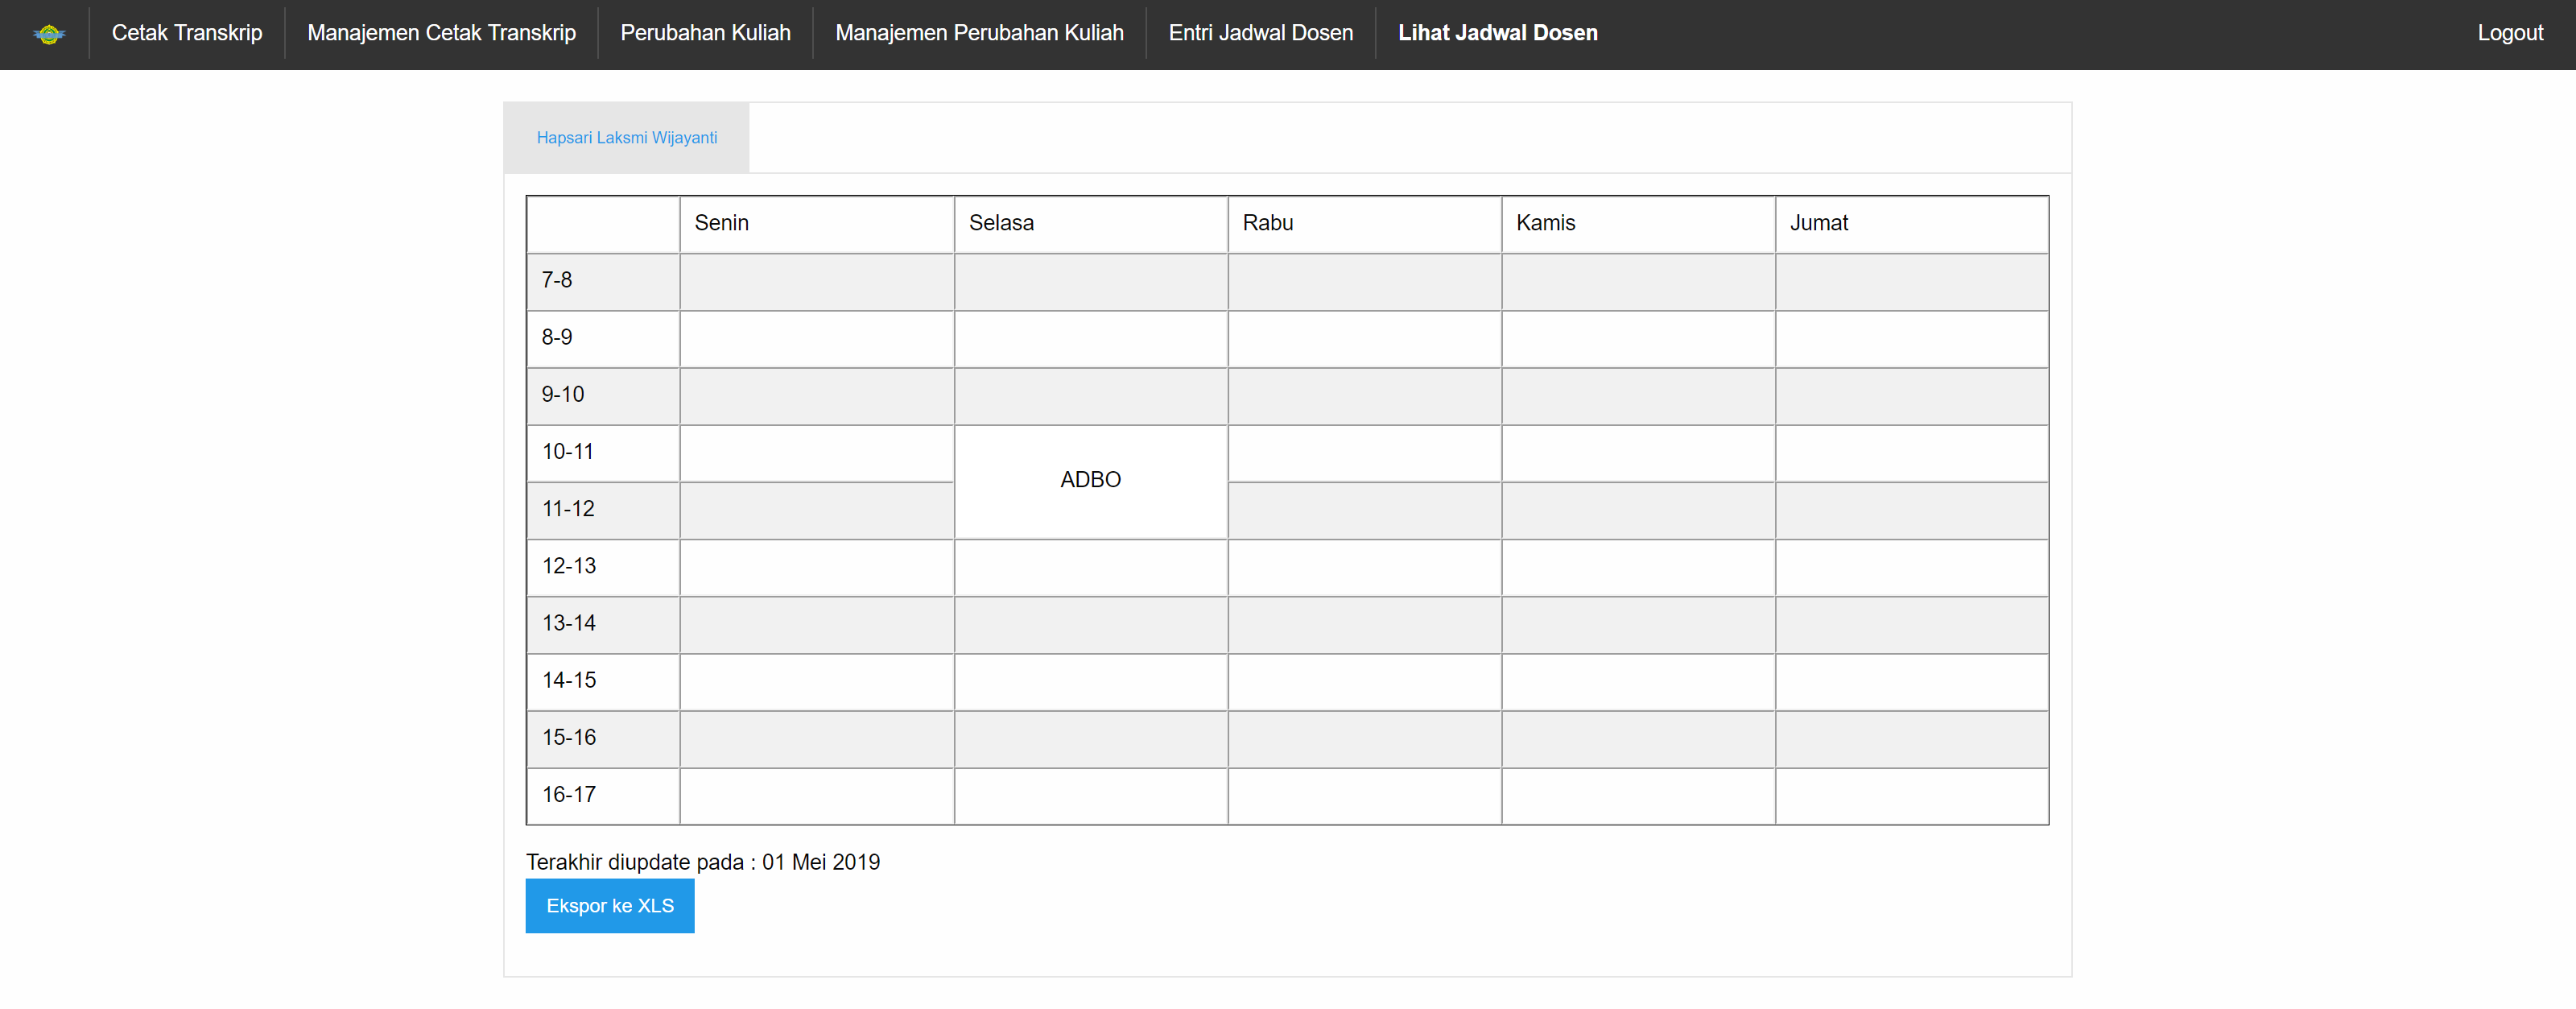
\includegraphics[scale=0.5]{Tampilan-Lihat-Jadwal-Dosen.png}  
	\caption{Struktur File Zurb Foundation} 	
\end{figure}
Tabel Jadwal Dosen akan \textit{retrieve} data jadwal dari setiap dosen yang dibuat. Seluruh mahasiswa dapat mengakses halaman ini. Terdiri dari rentang waktu dan hari. 
Lalu akan terlihat tanggal kapan terakhir jadwal bisa.